\section{Analiza porównawcza cech wybranych aplikacji mobilnych umożliwiających korzystanie z map} \label{roz:opis_srodowisk}

Dogłębna analiza rynku pozwoliła nam poznać istniejące już aplikacje mobilne umożliwiające nawigowanie po szlakach górskich oraz różne ich cechy, zarówno w wersji darmowej, jak i płatnej, premium. Poniższe porównanie  dwóch aplikacji pozwoliło na podjęcie decyzji, jak opisywana w tej pracy aplikacja powinna wyglądać.

\subsection{Platforma Mapa Turystyczna}
Aplikacja Mapa Turystyczna \cite{mapatu} jest to polska nakładka na Mapy Google. Wyznacza trasy tylko w ramach przebiegu szlaku wprowadzonego na mapy. Oprócz szlaków w Polsce, Czechach i Słowacji zaznaczone schroniska i niektóre atrakcje (np. jaskinie).

Rysunki 4.1 - 4.4 przedstawiają zrzuty ekranu z aplikacji mobilnej Mapa Turystyczna.
\begin{figure}[H]
    \centering
    \fbox{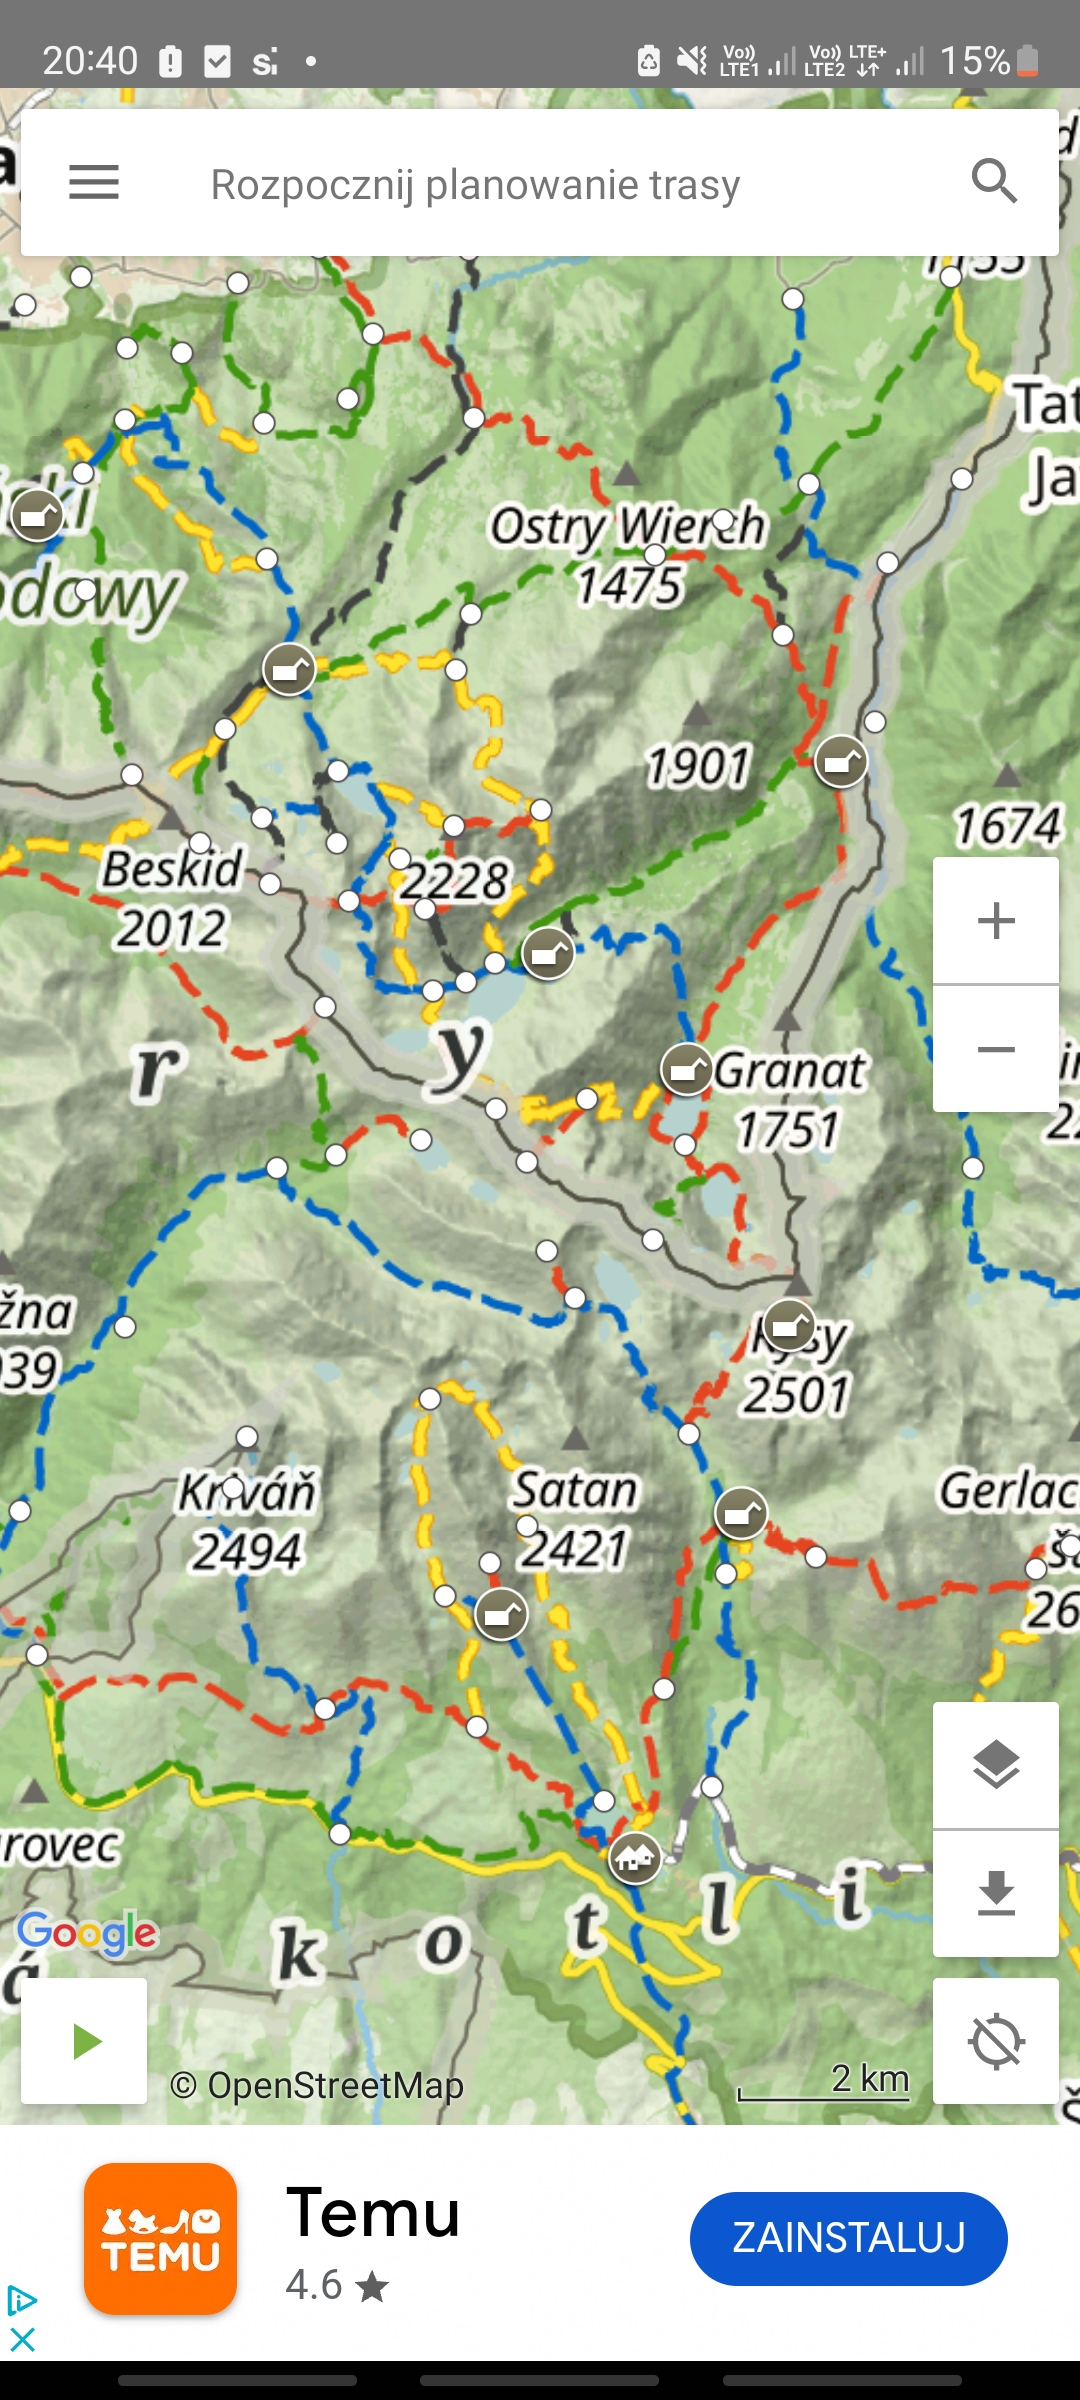
\includegraphics[scale=0.11]{img/rynek/mamatu-mapa.jpg}}
    \caption{Mapa Turystyczna - widok po uruchomieniu aplikacji.}
    \label{mapatu:mapa}
\end{figure}
Aplikacja mobilna po uruchomieniu przenosi od razu użytkownika do widoku prezentującego mapę. Domyślnie mapa ma wybraną warstwę zawierającą kolorowe szlaki turystyczne, jak i ścieżki rowerowe, zaznaczone na mapie bary, jadłodajnie, wodopoje oraz zabytki i inne miejsca warte zwiedzenia.

\begin{figure}[H]
    \centering
    \fbox{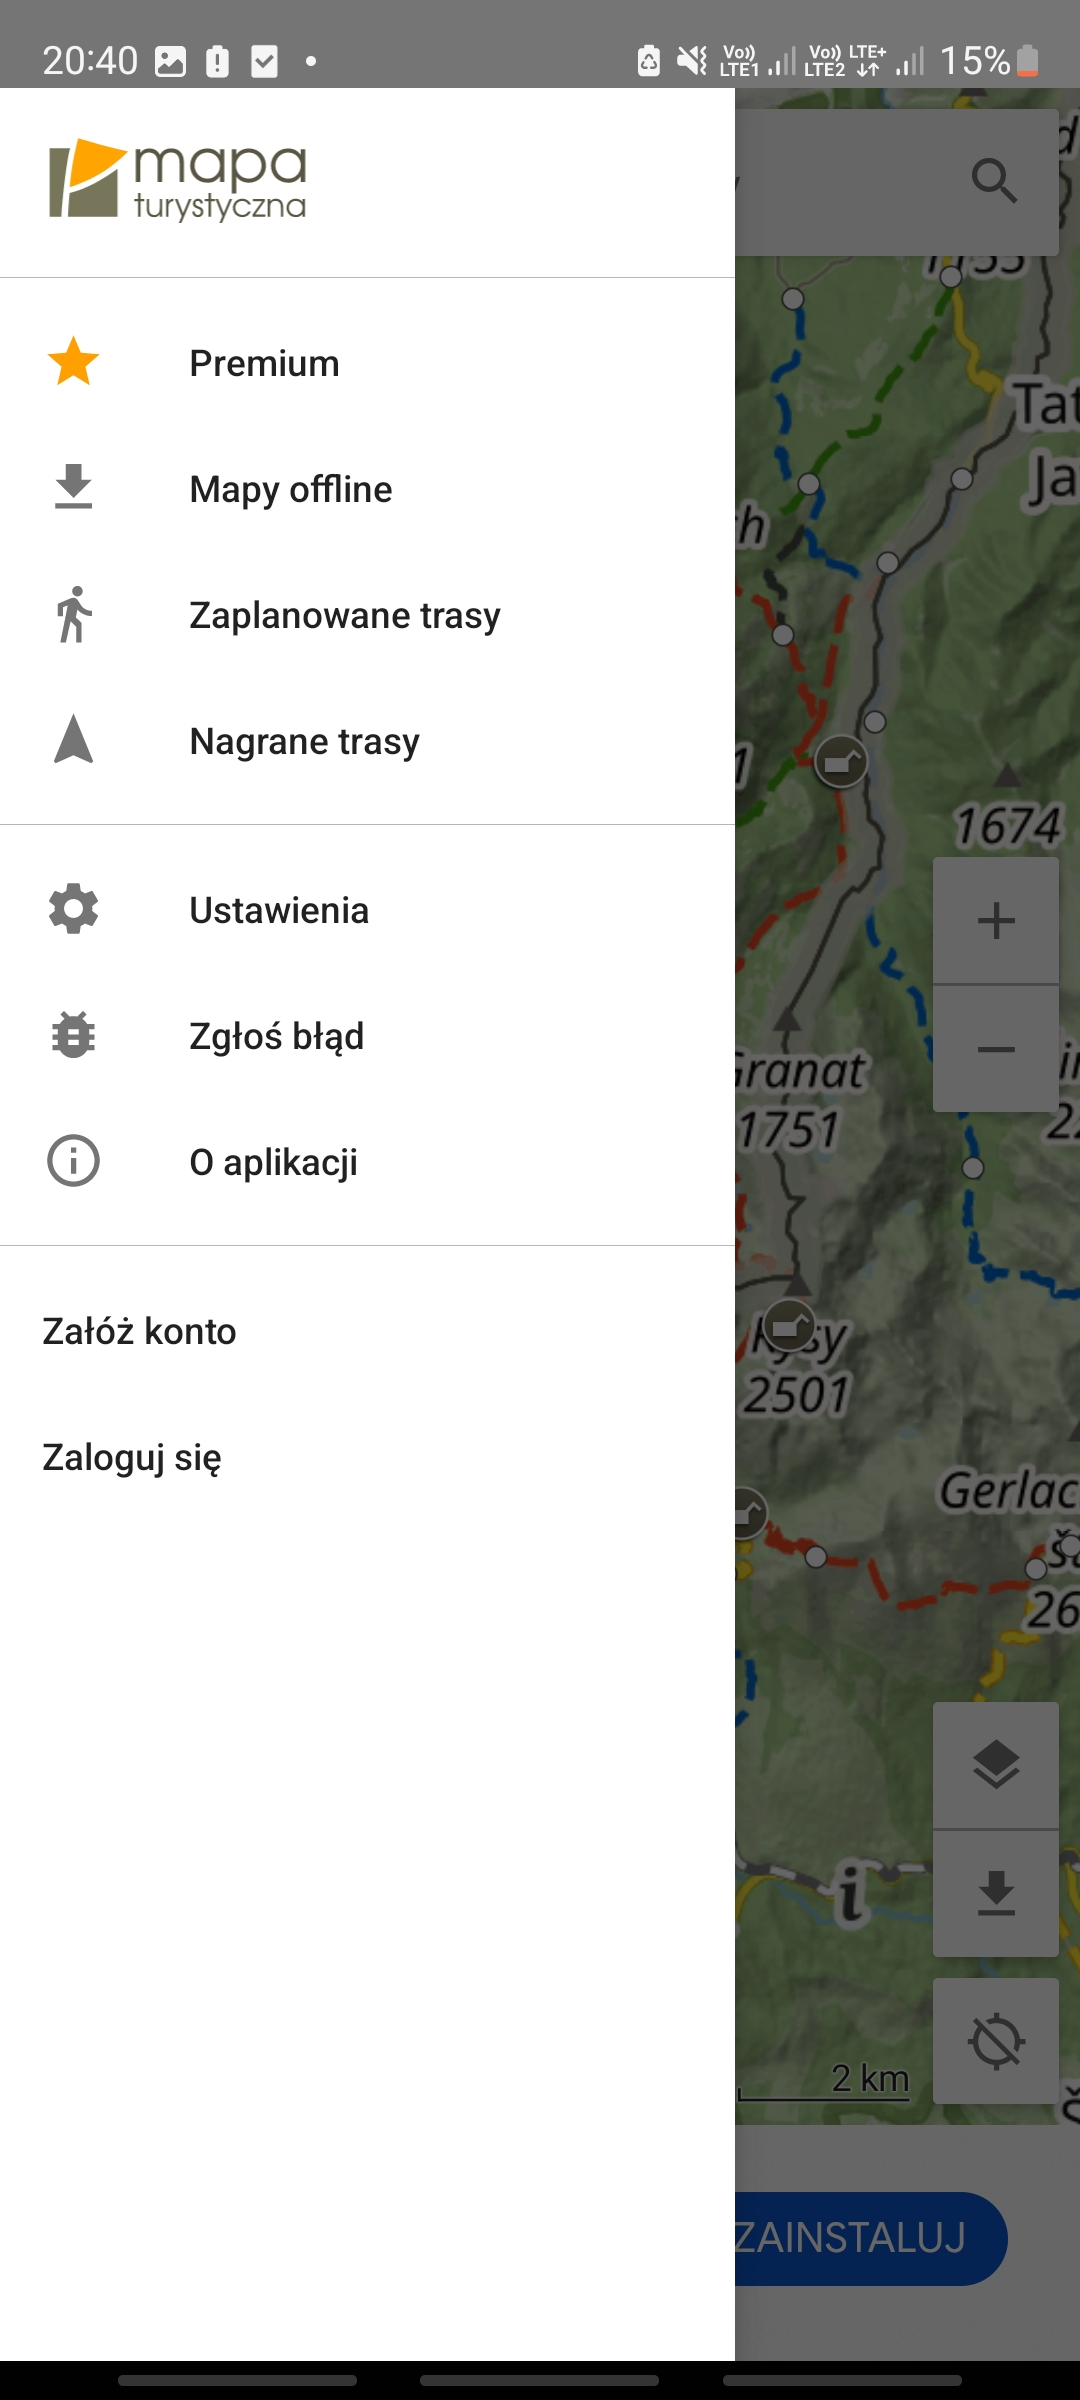
\includegraphics[scale=0.11]{img/rynek/mapatu-menu.jpg}}
    \caption{Mapa Turystyczna - menu z dostępnymi opcjami (użytkownik niezalogowany).}
    \label{mapatu:menu}
\end{figure}
Dostępne rozwijane menu z dodatkowymi opcjami. Opcja planowania trasy dostępna jest z wersji desktopowej aplikacji, a tak stworzoną mapę można zapisać na profilu jako użytkownik zalogowany i korzystać z niej na urządzeniu mobilnym. Przebyte trasy użytkownik może także nagrywać lub importować do aplikacji jako plik GPX w aplikacji webowej. Konieczne do tej funkcji jest założenie konta i zalogowanie użytkownika.
\begin{figure}[H]
    \centering
    \fbox{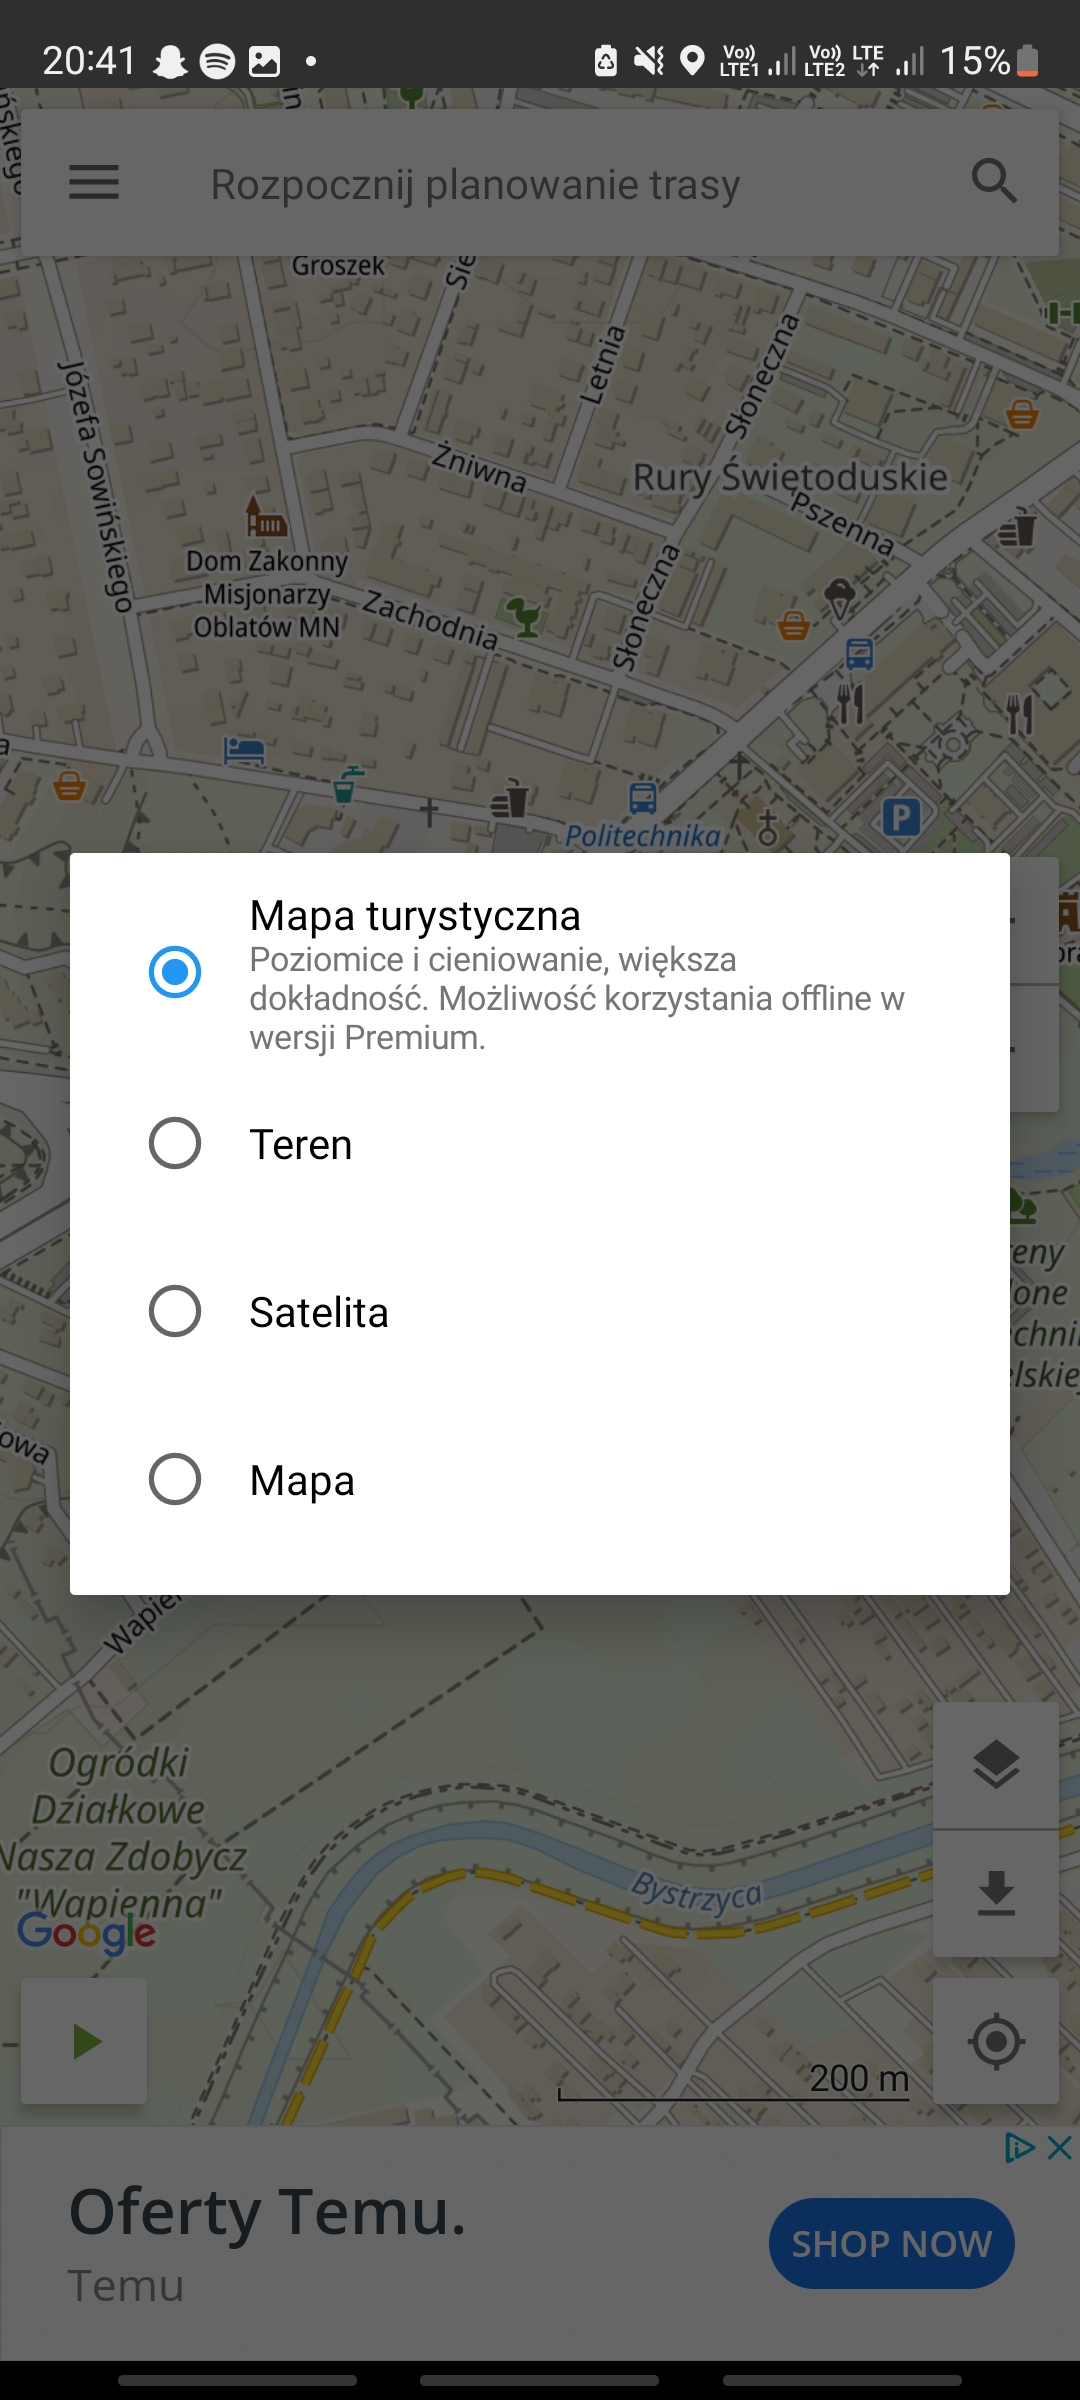
\includegraphics[scale=0.11]{img/rynek/mapatu-warstwy.jpg}}
    \caption{Mapa Turystyczna - dostępne warstwy mapy do wyboru.}
    \label{mapatu:warstwy}
\end{figure}
Na powyższym widoku przedstawione są dostępne warstwy mapy: satelita, mapa terenowa z zaznaczonymi terenami zielonymi oraz szlakami i żłobieniami w terenie oraz zwykła mapa. Pozwala to użytkownikowi na kontrolę tego, jakie informacje wyświetla jego aplikacja. 
\begin{figure}[H]
    \centering
    \fbox{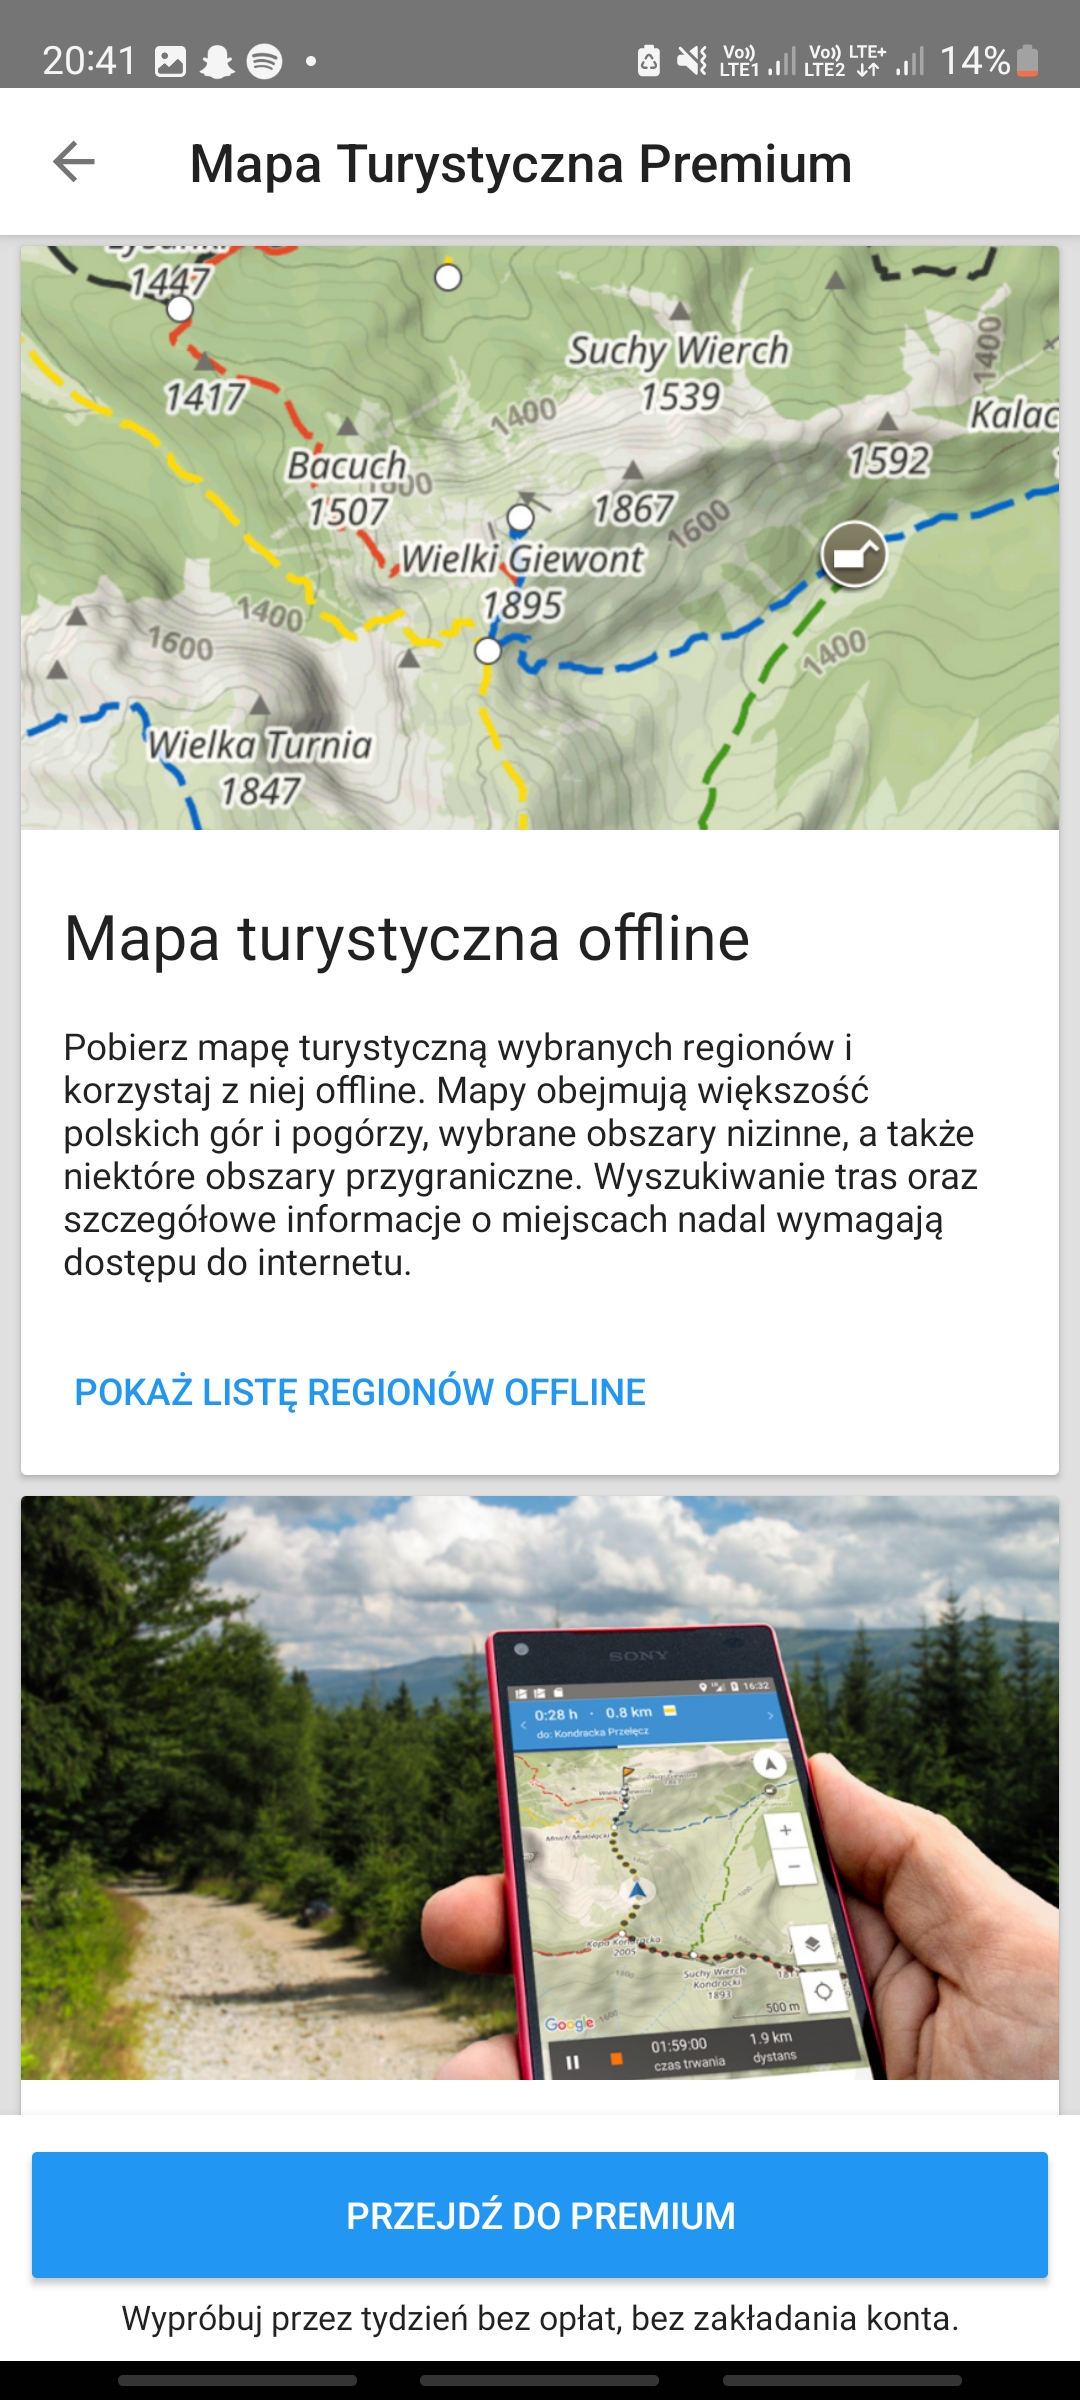
\includegraphics[scale=0.11]{img/rynek/mapatu-premium.jpg}}
    \caption{Mapa Turystyczna - dostępne funkcje po zakupie wersji premium.}
    \label{mapatu:premium}
\end{figure}
W wersji premium aplikacja mobilna oferuje nam wersję aplikacji bez uciążliwych reklam, nawigację po trasie, nakładanie własnych tras na mapę a także pobieranie map i korzystanie z nich w trybie offline.

\textbf{Wady}
\begin{itemize}
    \item Pełna wersja aplikacji płatna (miesiąc 8zł, rok – 35zł).
    \item W darmowej wersji mapy nie działają bez sieci komórkowej.
    \item Nie można dodać własnych map.
    \item Gotowe mapy nie obejmują terytorium Ukrainy.
    \item Wersja darmowa zawiera dużo reklam.
    \item Brak powiadomień o zagrożeniach.
    \item Nie tworzy trasy, użytkownik idzie po mapie, bez nawigacji.
\end{itemize}
\textbf{Zalety}
\begin{itemize}
    \item Dostępny darmowy tydzień testowy, dzięki któremu można pobrać mapy offline.
    \item Prosta obsługa.
    \item Oprócz trasy w wyniku planowania otrzymujemy: profil, czas przejścia, informację o punktach GOT.
    \item Aplikacja mobilna i wersja desktopowa.
    \item Historia tras oraz możliwość planowania podróży z wyprzedzeniem.
\end{itemize}

\subsection{Platforma Mapy.cz}
Aplikacja Mapy.cz \cite{mapycz} rozwijana w wielu językach, darmowa, bez konieczności logowania. Po ówczesnej rejestracji użytkownik ma możliwość zapisywania tras i dodawania zdjęć obiektów spotkanych na swojej drodze. Oprócz wyszukiwania tras aplikacja oferuje także wyszukiwanie atrakcji, nawigację i mapy offline. Podczas planowania trasy istnieje możliwość jej zapisania i udostępniania, a także dodanie do niej interesujących obiektów. Bez aplikacji mobilnej istnieje możliwość odczytania współrzędnych z mapy webowej.

Rysunki 4.5 - 4.8 przedstawiają zrzuty ekranu z aplikacji mobilnej Mapy.cz.
\begin{figure}[H]
    \centering
    \fbox{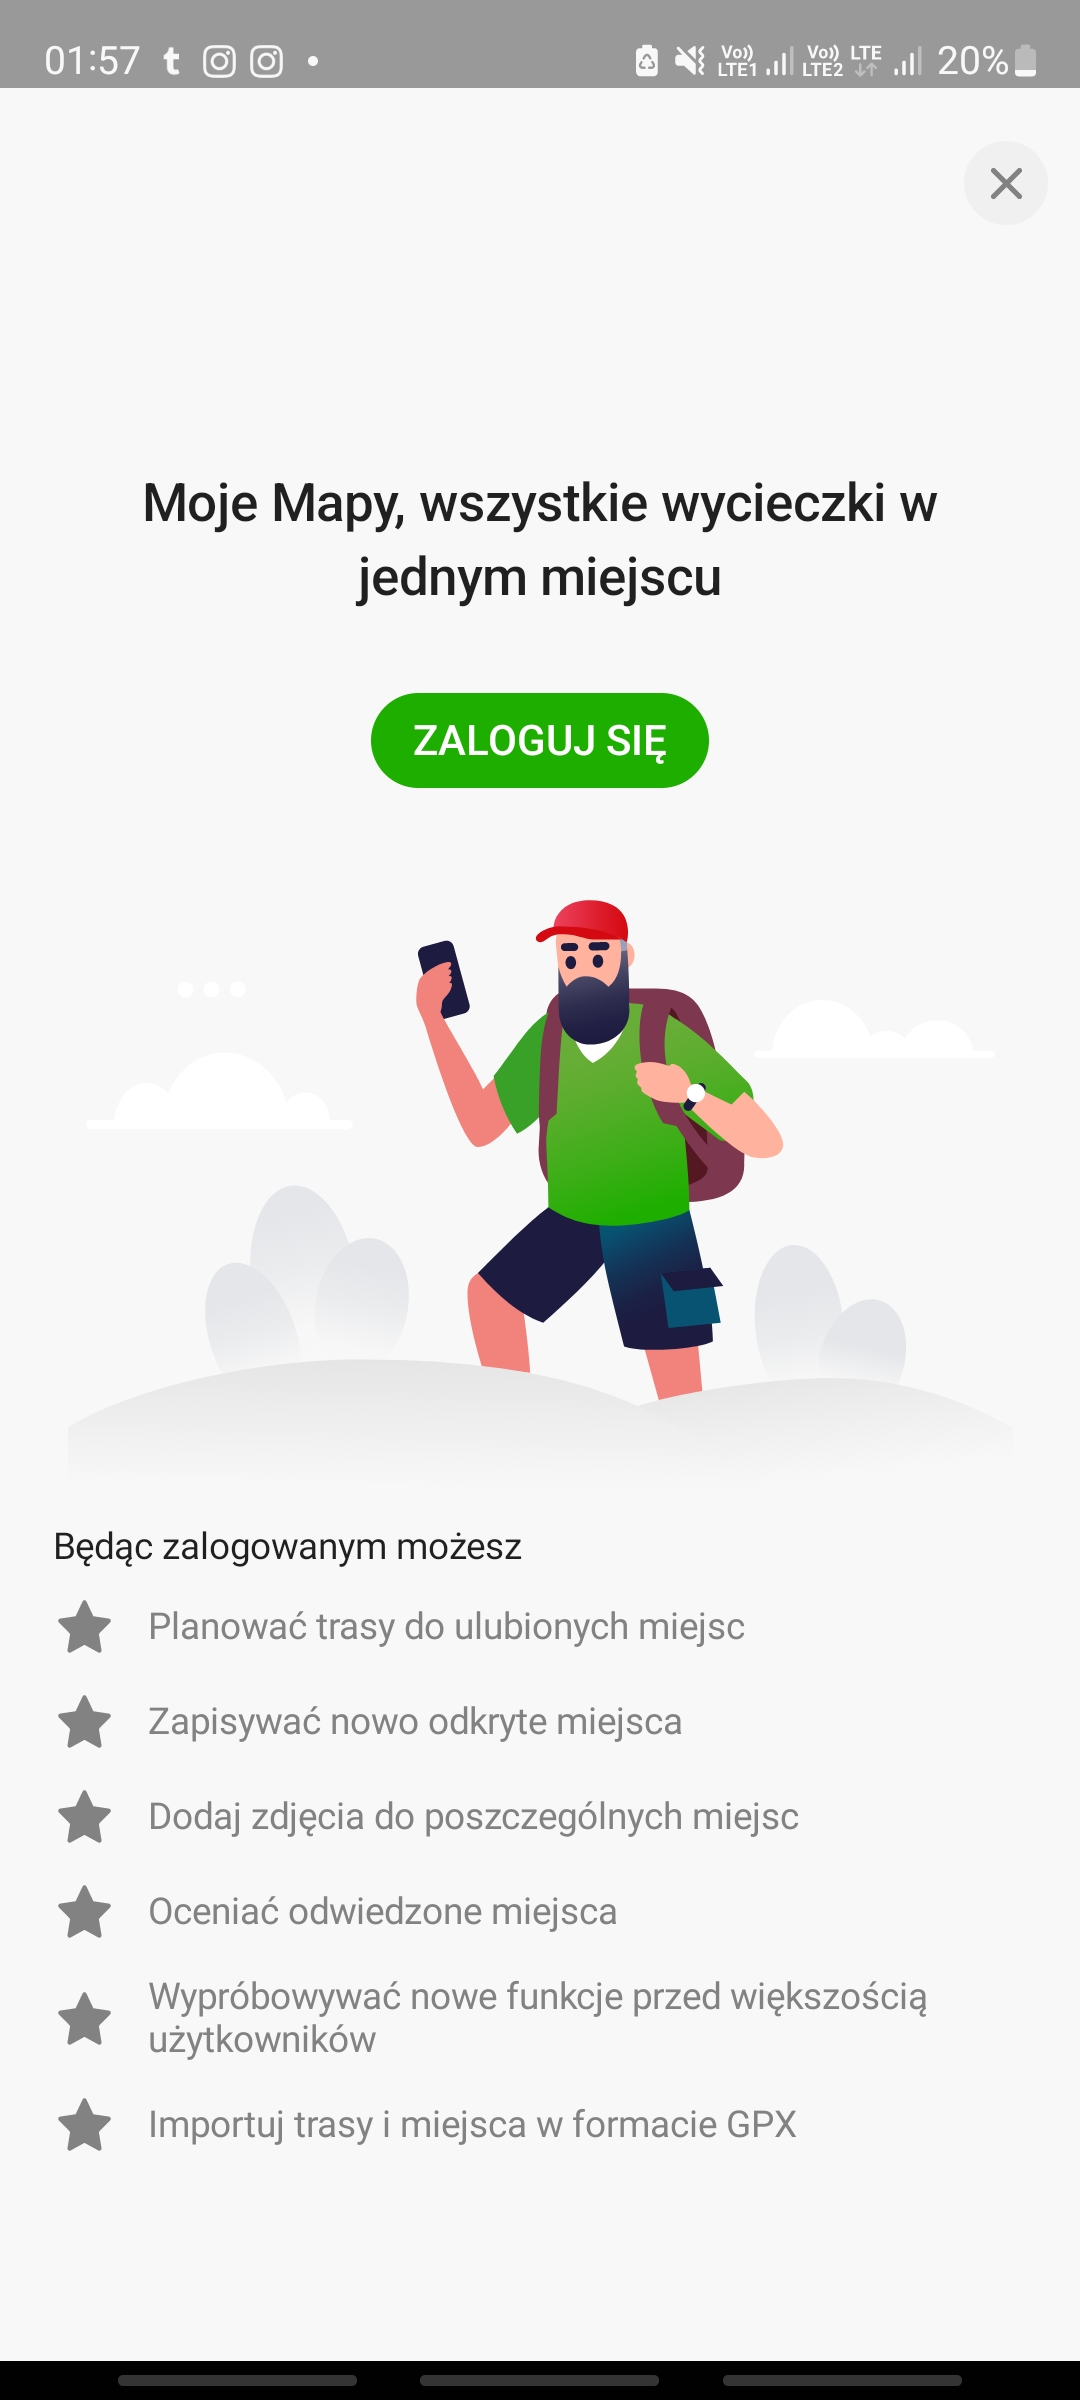
\includegraphics[scale=0.11]{img/rynek/Mapycz_logowanie.jpg}}
    \caption{Mapy.cz - funkcje dostępne po założeniu konta.}
    \label{mapycz:logowanie}
\end{figure}
Aplikacja po uruchomieniu po raz pierwszy wita użytkownika powyższym widokiem. Przedstawione są na nim dodatkowe funkcje dostępne dopiero po zalogowaniu do aplikacji. Te funkcje to m.in. planowanie i zapisywanie trasy oraz ciekawych miejsc, dodawanie zdjęć ze szlaku, ocenianie odwiedzonych miejsc oraz import tras i miejsc w formacie GPX. 
\begin{figure}[H]
    \centering
    \fbox{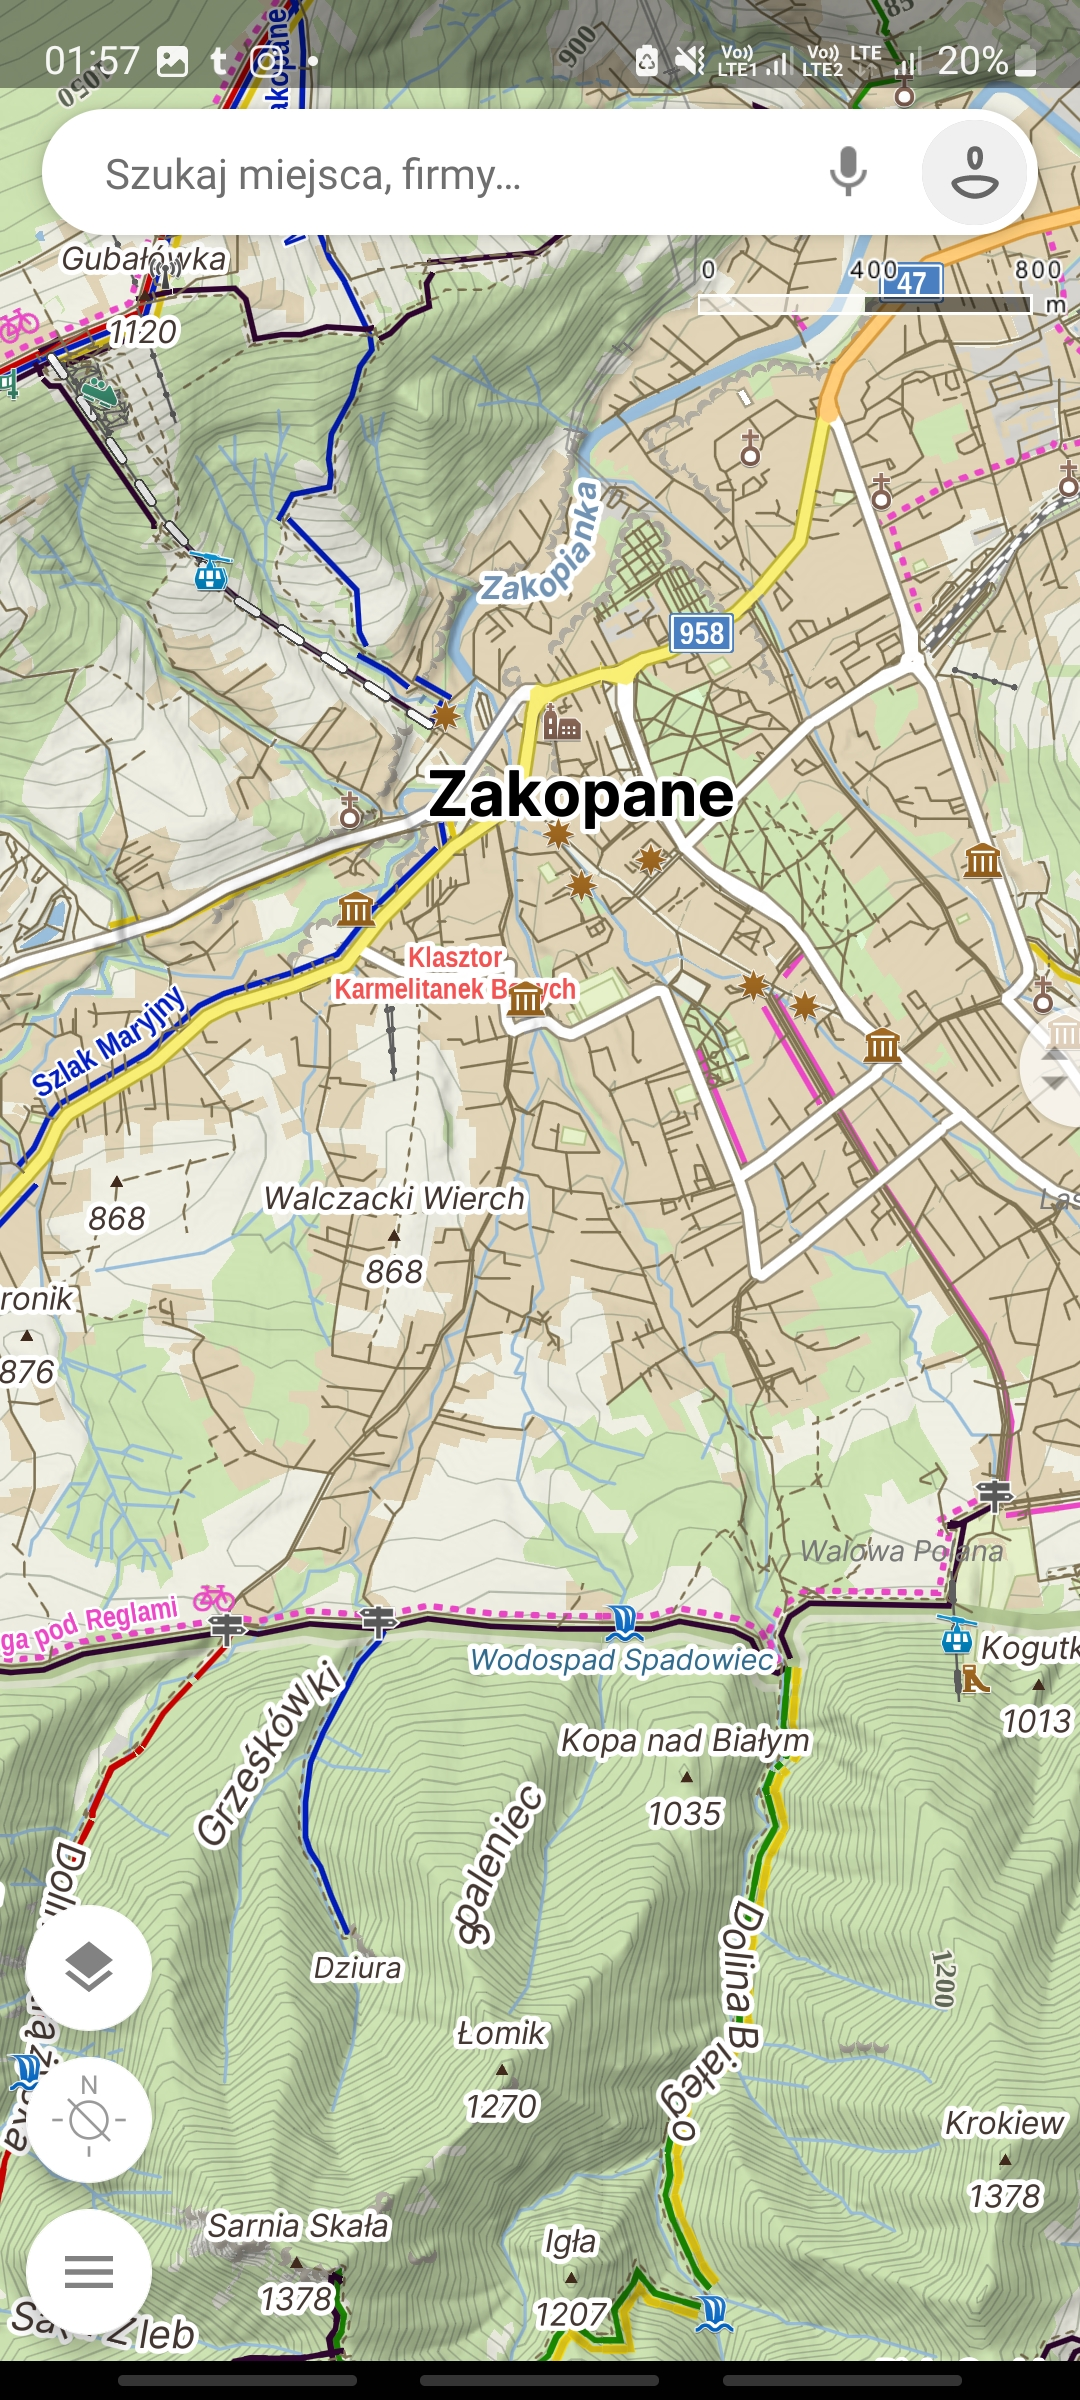
\includegraphics[scale=0.11]{img/rynek/Mapycz_glowna.jpg}}
    \caption{Mapy.cz - widok główny.}
    \label{mapycz:glowna}
\end{figure}
Kolejnym widokiem jest ekran główny, którego dominującym elementem jest skalowalna mapa, na której oprócz szlaków zaznaczone są także atrakcje turystyczne. Na górze ekranu ukazana jest wyszukiwarka miejsc na mapie. W lewym dolnym rogu widoczne są trzy przyciski: zmiana typu mapy (rys. \ref{mapycz:mapy}), lokalizacja oraz rozwijane menu.  W dostępnym po kliknięciu w ikonę menu znajdują się takie funkcje, jak: dostęp do konta, moje mapy, planuj trasę, wycieczka po okolicy, mapy offline, udostępnij lokalizację, uruchom rejestrator i ustawienia, a także skróty do mediów społecznościowych twórców i pierwsza pomoc (rys. \ref{mapycz:pomoc}).
\begin{figure}[H]
    \centering
    \fbox{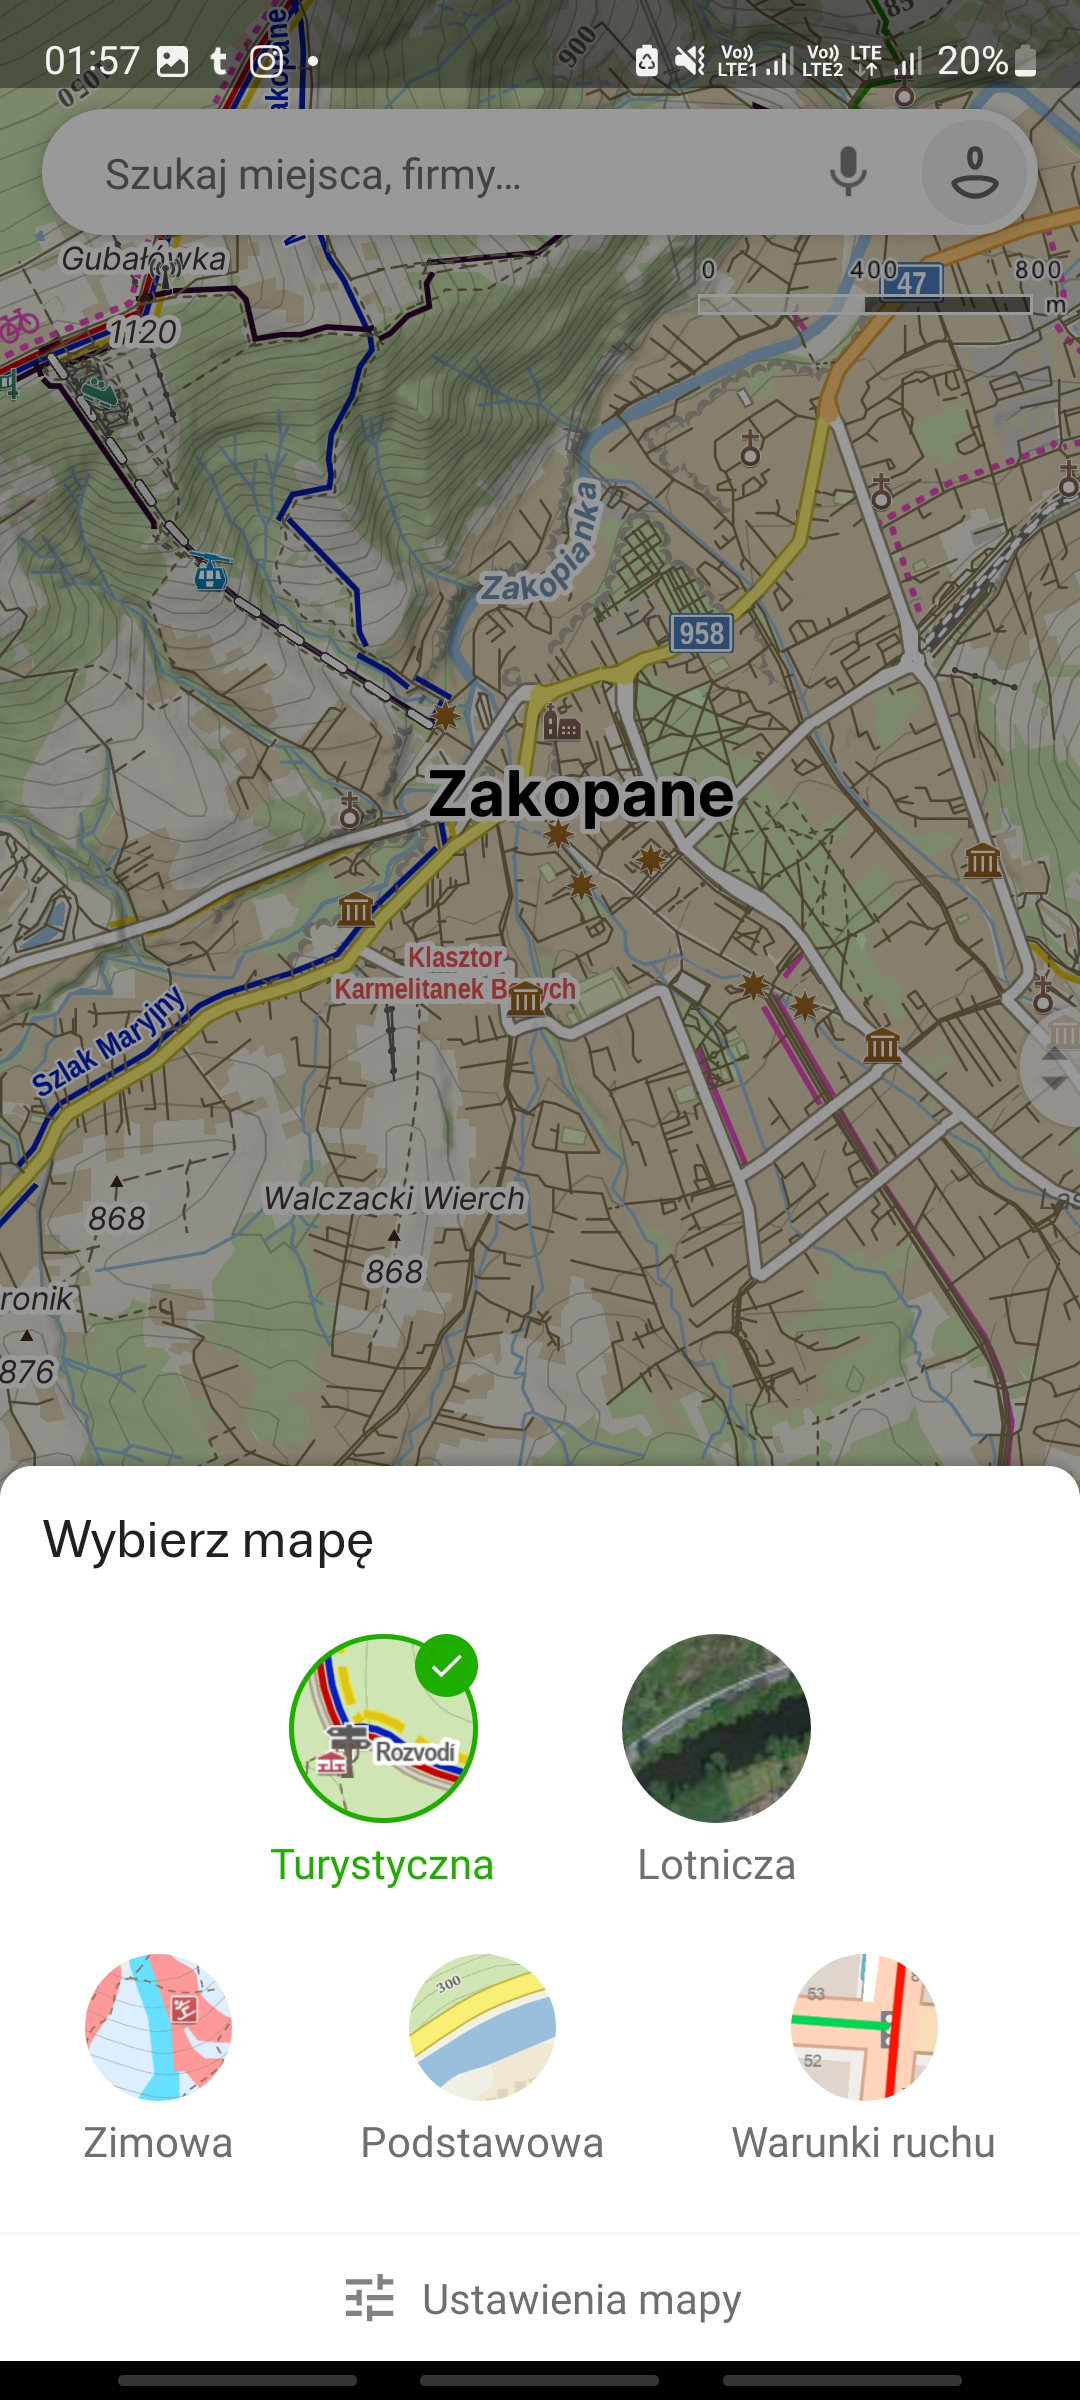
\includegraphics[scale=0.11]{img/rynek/Mapycz_mapy.jpg}}
    \caption{Mapy.cz - dostępne typy map.}
    \label{mapycz:mapy}
\end{figure}
Na rysunku \ref{mapycz:mapy} widać dostępne typy map oferowane przez aplikację. Domyślnie typ mapy ustawiony jest na "turystyczna" z zaznaczonymi szlakami górskimi, lecz do wyboru użytkownik ma także: lotniczą, zimową, podstawową oraz warunki ruchu. W zależności od potrzeb użytkownika może on swobodnie wybierać różne tryby mapy. 
\\
\begin{figure}[H]
    \centering
    \fbox{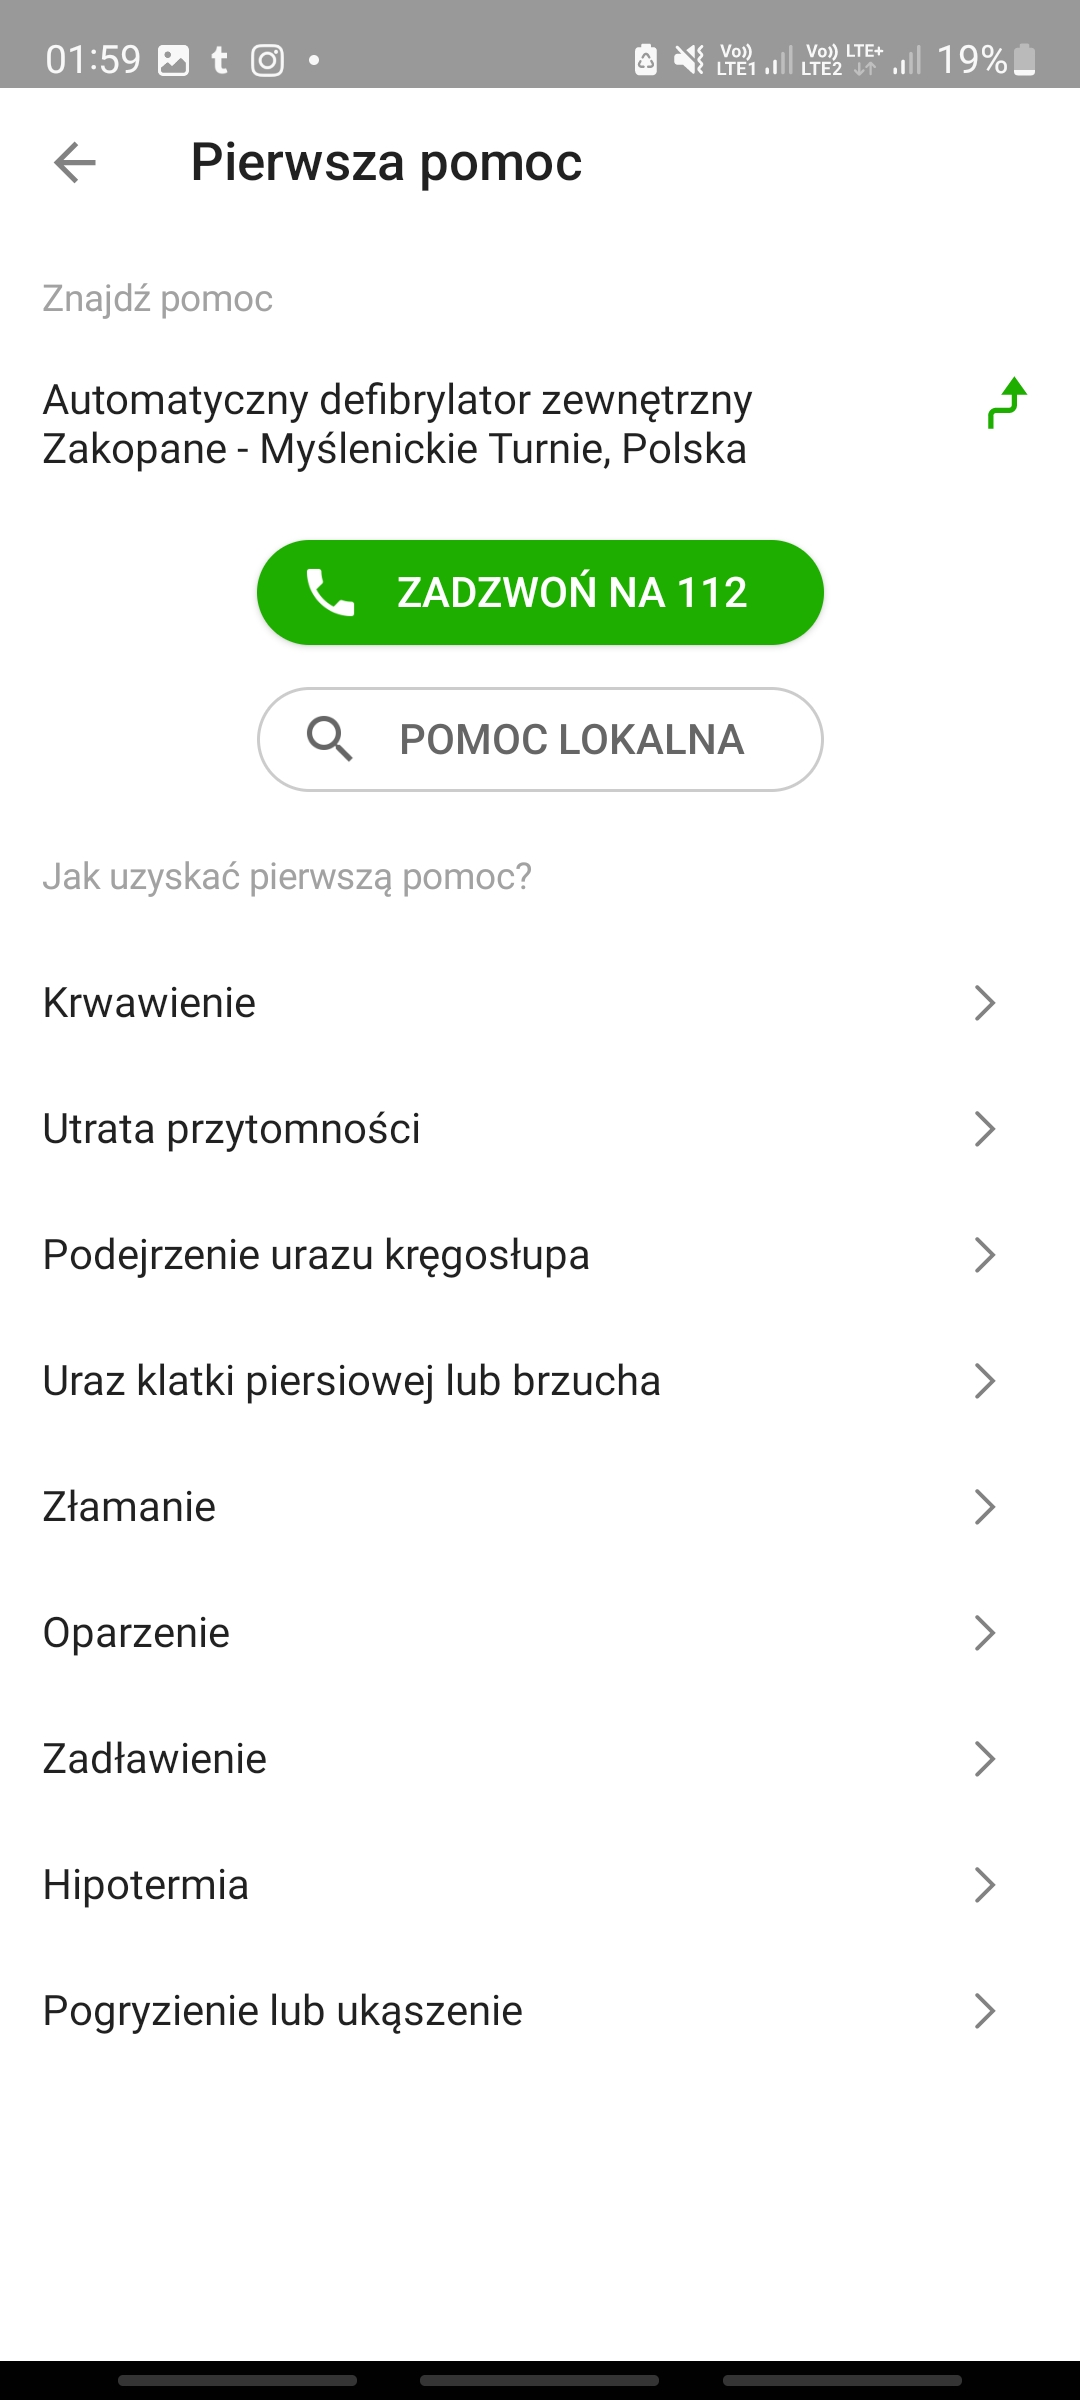
\includegraphics[scale=0.11]{img/rynek/Mapycz_pomoc.jpg}}
    \caption{Mapy.cz - widok zawierający wskazówki dotyczące pierwszej pomocy.}
    \label{mapycz:pomoc}
\end{figure}
Powyższy widok zawiera wiele przydatnych opcji w razie wypadku na szlaku. Na samej górze opcja szukania najbliższego defibrylatora AED, możliwość nawigacji do punktu, w którym się znajduje. Poniżej znajdują się przyciski do bezpośredniego dzwonienia na numer 112 i przycisk do szukania pomocy lokalnie podpowiadający najbliższe szpitale i cenrta pomocy z opcją naprowadzania do nich. Większą część tego widoku zajmują przyciski z opisanymi możliwymi urazami, po kliknięciu których użytkownik zostaje przeniesiony do widoku odpowiadającemu danemu urazowi z instrukcjami, również graficznymi, jak postąpić w danej sytuacji.

\textbf{Wady}
\begin{itemize}
    \item Wyszukiwanie w polu tekstowym nie do końca dopracowane.
    \item Słaba nawigacja po aplikacji - wybór jednej opcji niweluje możliwość powrotu do ostatniego miejsca; jeżeli użytkownik po wybraniu którejś opcji przejdzie do ekranu głównego, to musi on ponownie szukać poprzednio przeglądanego ekranu.
\end{itemize}
\textbf{Zalety}
\begin{itemize}
    \item Łatwa w obsłudze, przypomina Mapy Google.
    \item Pobieranie map offline (region lub cały kraj).
    \item Płynność działania.
    \item Łatwe planowanie trasy z dużą liczbą punktów pośrednich.
    \item Możliwość rejestrowania trasy.
    \item W pełni darmowa aplikacja mobilna i webowa.
\end{itemize}



